\section{Birth 두 sector의 엄밀한 부호}\label{sec:birth}
실제 endpoint의 공통 평균 adjoint는 $\overline z_x<0$, $\overline z_w>0$을 만족한다. 필요한 componentwise 포함은
\begin{align}
\overline z_x&\in[-49430.25337661141,-48867.81791954700],\\
\overline z_w&\in[7735.849570431344,7735.908522222911],\\
\overline z^{\mathsf T}\nu_{24}&\in[-48644.55871834544,-48082.11727381872].
\label{eq:zsign}
\end{align}
이 행벡터의 단위는 $n_T$와 같이 각 gas 성분당 K다. 식 \eqref{eq:adjointrow}에서 계산한 weighted row 보정 상계는 $8.470521103361278\times10^{-7}$ K이며, 식 \eqref{eq:zsign}에는 그 오차가 이미 들어 있다.\cite{endpoint16}

수송의 아래 node로 가는 coefficient를 $\alpha^R_{24}=(1-\rho)E_{24}/(E_{24}-E_{23})>0$라 쓰자. 이는 fixed-source 선택을 가리키는 $\alpha$와 구별된다. $\beta_j=\tau_j/(1+\tau_j)^2$라 두면 원 두 birth sector의 유한 온도 기여는
\begin{align}
\frac{\Delta T_{bR}}b&=
\frac{M_\gamma\alpha^R_{24}}{\Pi_F}\bigl[
(\beta_{23}-\beta_{24})\overline z_x
+(\epsilon_{23}\beta_{23}-\epsilon_{24}\beta_{24})\overline z_w\bigr],\label{eq:birthR}\\
\frac{\Delta T_{bBE}}b&=-\frac{M_\gamma C_{1,24}}{\Pi_F}
\overline z^{\mathsf T}\nu_{24}.
\label{eq:birthBE}
\end{align}
여기서 $b>0$이며 $b=0$에서는 두 항이 정확히 0이다. 식의 비율은 같은 전체 endpoint에서 정의한 sector 기여를 $b$로 나눈 값이다. 전체 해의 $b$에 대한 매개변수 미분과는 다른 관측량이다.

\subsection{작은 coefficient 차이의 인수 분해}
$\eta=hc n_2(1-x_2)$, $\tau_j=\eta\sigma_j$로 두면
\begin{equation}
\beta_{23}-\beta_{24}
=\frac{\eta(\sigma_{23}-\sigma_{24})(1-\eta^2\sigma_{23}\sigma_{24})}
{(1+\eta\sigma_{23})^2(1+\eta\sigma_{24})^2}>0.
\label{eq:dbeta}
\end{equation}
Heat coefficient의 차이는 $A=\epsilon_{23}\sigma_{23}$, $B=\epsilon_{24}\sigma_{24}$로 두어
\begin{equation}
\epsilon_{23}\beta_{23}-\epsilon_{24}\beta_{24}
=\frac{\eta[(A-B)+2\eta(A\sigma_{24}-B\sigma_{23})
+\eta^2(A\sigma_{24}^2-B\sigma_{23}^2)]}
{(1+\eta\sigma_{23})^2(1+\eta\sigma_{24})^2}
\label{eq:dheat}
\end{equation}
로 먼저 정리했다. 원 captured leaf에서 분자의 세 coefficient는 모두 음수다. 실제 포함은
\begin{align}
\beta_{23}-\beta_{24}&\in[2.360824014240304,2.464667889011005]\times10^{-6},\\
\epsilon_{23}\beta_{23}-\epsilon_{24}\beta_{24}
&\in[-1.234357139375600,-1.182248199814379]\times10^{-5}\ \mathrm{eV}.
\label{eq:birthdiffvalues}
\end{align}
각 큰 coefficient를 독립 구간으로 만든 뒤 빼면 사라질 수 있는 상쇄를 식 \eqref{eq:dbeta}--\eqref{eq:dheat}가 보존한다.

\begin{proposition}[실제 birth 부호]\label{prop:birthsign}
현재 같은 COMMON의 fixed-source 계열 전체와 $0<b\le1$에서
\begin{equation}
\Delta T_{bR}<0,\qquad \Delta T_{bBE}>0,
\qquad \Delta T_{bR}+\Delta T_{bBE}>0.
\label{eq:birthsign}
\end{equation}
\end{proposition}
\begin{proof}
식 \eqref{eq:birthR}에서 두 괄호 항은 식 \eqref{eq:zsign}, \eqref{eq:birthdiffvalues}에 의해 각각 음수다. 식 \eqref{eq:birthBE}에서는 $M_\gamma,C_{1,24},\Pi_F$가 양수이고 $\overline z^{\mathsf T}\nu_{24}<0$이므로 전체가 양수다. 아래 실제 구간에서 양의 두 번째 항의 하한이 첫 번째 항의 절댓값 상한보다 크므로 합도 양수다.
\end{proof}

\begin{table}[H]
\centering\small
\begin{tabular}{@{}lrr@{}}
\toprule
유한 sector 비율 [K] & 하한 & 상한\\\midrule
$\Delta T_{bR}/b$ & $-2.193573619033929\times10^{-9}$ & $-2.084075101148286\times10^{-9}$\\
$\Delta T_{bBE}/b$ & $6.795510419222985\times10^{-5}$ & $7.189758987952319\times10^{-5}$\\
\bottomrule
\end{tabular}
\caption{$b>0$에서의 실제 포함. $b=0$을 포함한 계열에서는 첫 항이 $[-2.193573619033929\times10^{-9},0]$ K, 두 번째 항이 $[0,7.189758987952319\times10^{-5}]$ K다.}
\label{tab:birth}
\end{table}

\section{실제 endpoint와 광자 관측량}\label{sec:results}
\subsection{기체 차이와 나머지의 크기}
표 \ref{tab:gasresults}의 gas 차이는 모든 $\lambda,b\in[0,1]$를 포함한다. $g_2$와 $g_F$를 각자 새로 풀거나 큰 구간 두 개를 독립적으로 빼서 얻지 않았다. 식 \eqref{eq:r}의 작은 잔차를 원 $C,B$로 전달한 뒤 식 \eqref{eq:intersection}을 교차했다. 모든 이온 fraction의 차이는 양수이고, thermal energy와 온도의 차이는 음수다. $w$ 감소와 전자 수 증가가 온도 분자에서 같은 음의 방향으로 작용한다.\cite{app16,endpoint16}

\begin{table}[H]
\centering\small
\begin{tabular}{@{}lrr@{}}
\toprule
관측량 & 하한 & 상한\\\midrule
$d_x$ & $4.968079869744687\times10^{-8}$ & $6.424793358338289\times10^{-8}$\\
$d_{y_1}$ & $1.673464100458090\times10^{-11}$ & $2.398033044762938\times10^{-11}$\\
$d_{y_2}$ & $1.261950768712229\times10^{-12}$ & $1.455327137828615\times10^{-12}$\\
$d_w$ [eV/H] & $-2.378772061684228\times10^{-8}$ & $-1.828217232284575\times10^{-8}$\\
$\Delta e$ [electrons/H] & $4.968232944627\times10^{-8}$ & $6.425017521665\times10^{-8}$\\
$\Delta n_e$ [cm$^{-3}$] & $4.944257155952\times10^{-12}$ & $6.394011555549\times10^{-12}$\\
$\Delta T$ [K] & $-1.585967387181453\times10^{-3}$ & $-1.210819969055199\times10^{-3}$\\
\bottomrule
\end{tabular}
\caption{같은 COMMON의 Full 대비 two-half 유한 차이. $d$와 $\Delta T$는 endpoint 교차 후의 포함이며, $\Delta e,\Delta n_e$는 잔차 적용 run01에서 이미 확보한 유효한 포함을 유지했다. 마지막 두 전자 관측량을 추가로 좁히는 계산은 필요하지 않았다.}
\label{tab:gasresults}
\end{table}

실제 $D_0$에서 얻은 반경과 교차 뒤 반경은 각각
\[
a\le4.283196217660632\times10^{-6},\qquad
a_{new}\le4.283195572225527\times10^{-6}
\]
이다. 표 \ref{tab:tails}은 원래의 더 큰 $a$로 계산했으므로 최종 포함에도 유효하다. 이론 나머지는 약 $10^{-12}$ K로, 표 \ref{tab:gasresults}의 계열 온도 폭 $3.7515\times10^{-4}$ K보다 약 여덟 자릿수 작다. 따라서 현재 결과 폭의 주원인은 endpoint 이차 전달을 생략해서 생기는 오차가 아니라, 계열 전체의 입력 구간과 남은 의존성 손실이다.

\begin{table}[H]
\centering\small
\begin{tabularx}{\textwidth}{@{}X r@{}}
\toprule
명시적 나머지 ($m=2$) & 외향 상한\\\midrule
유한 선형 tail $q^3a$ & $6.925011124851535\times10^{-18}$\\
곡률 항 $\tfrac12L_Ha^2(1+q+q^2)$ & $7.594228219947642\times10^{-16}$\\
전체 scaled endpoint 반경 $\epsilon_2$ & $7.663478331196157\times10^{-16}$\\
정확한 endpoint Newton 전달과의 차이 & $7.594228219959920\times10^{-16}$\\
온도 분자 $N_T$ 오차 [K] & $3.627645274572929\times10^{-12}$\\
같은 $\Pi_F$에서의 $\Delta T$ 오차 [K] & $1.710575696736044\times10^{-12}$\\
\bottomrule
\end{tabularx}
\caption{식 \eqref{eq:quadbound}, \eqref{eq:eps}, \eqref{eq:goalerror}의 실제 적용. 마지막 행은 계열 온도 자체의 폭이나 실측 불확실도를 뜻하지 않는다.}
\label{tab:tails}
\end{table}

\subsection{같은 응답을 거친 물리 sector}
표 \ref{tab:sectors}과 그림 \ref{fig:sectors}은 같은 $\overline A^{-1}$와 $\Pi_F$를 적용한 유한 기여다. Stock BE의 음의 기여는 약 $0.82$--$0.91$ mK이고 opacity 변화의 기여는 약 $0.43$--$0.45$ mK로, 현재 계열에서 가장 크다. Gas movement도 약 $0.13$--$0.16$ mK의 음의 기여를 보탠다. Birth BE의 양의 기여는 $b=1$에서도 약 $0.068$--$0.072$ mK여서 전체 음의 온도 차이를 뒤집지 않는다.

\begin{table}[H]
\centering\small
\begin{tabular}{@{}lrr@{}}
\toprule
Sector [K] & 하한 & 상한\\\midrule
Source 시각 & $-4.743893361686294\times10^{-6}$ & $-4.063113430475724\times10^{-6}$\\
Gas movement & $-1.560191742487882\times10^{-4}$ & $-1.331095358067088\times10^{-4}$\\
Opacity 변화 & $-4.544065812945129\times10^{-4}$ & $-4.253826526597355\times10^{-4}$\\
흡수·수송 순서 & $-1.531798755376485\times10^{-8}$ & $-1.384519131043111\times10^{-8}$\\
Stock 중간 수송 & $-6.306644704453658\times10^{-5}$ & $9.693239716841109\times10^{-5}$\\
Stock BE & $-9.054110638002102\times10^{-4}$ & $-8.180893260372340\times10^{-4}$\\
Remap 합성 & $-6.332389760132570\times10^{-7}$ & $1.443360409610727\times10^{-6}$\\
Birth 수송, $0\le b\le1$ & $-2.193573619033929\times10^{-9}$ & $0$\\
Birth BE, $0\le b\le1$ & $0$ & $7.189758987952319\times10^{-5}$\\
\bottomrule
\end{tabular}
\caption{공통 adjoint 나머지를 포함한 실제 sector 온도 구간. 두 birth 행은 식 \eqref{eq:birthR}--\eqref{eq:birthBE}의 구조적 인수 분해를 추가 사용했다.}
\label{tab:sectors}
\end{table}

\begin{figure}[H]
\centering
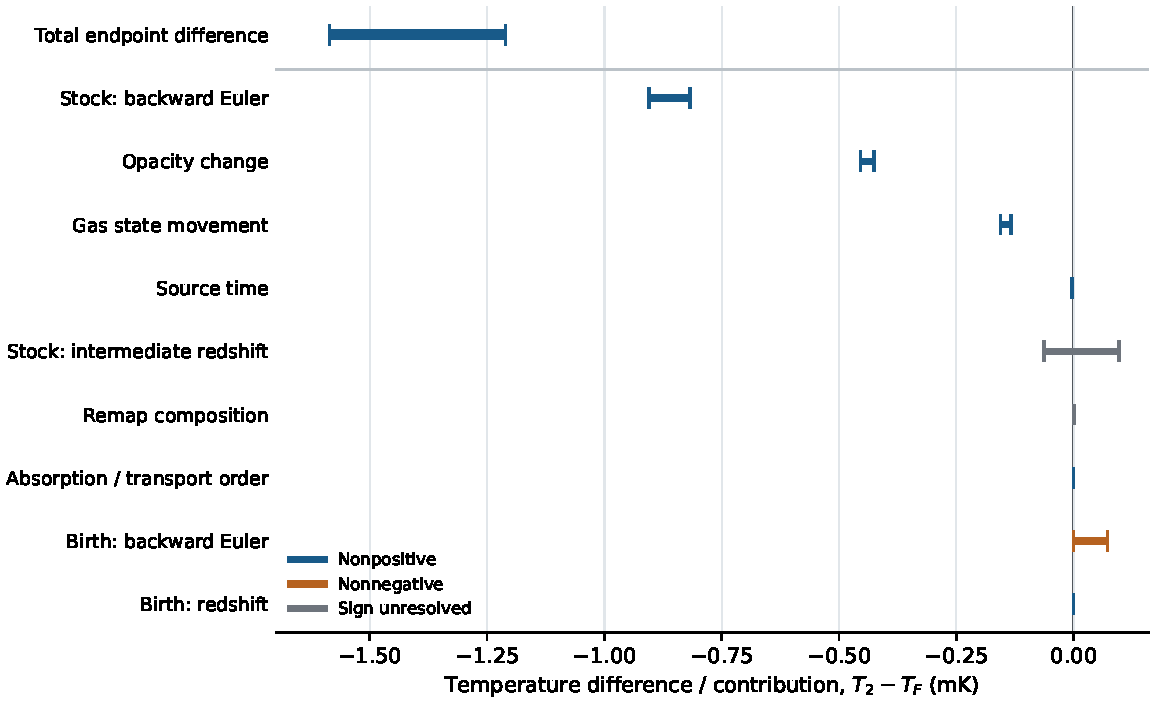
\includegraphics[width=\textwidth]{temperature_sectors.pdf}
\caption{계열 전체의 결정론적 외향 포함이며 통계적 신뢰구간이 아니다. 각 sector에 같은 inverse와 온도 분모를 적용했고 $b=0$을 포함했다. 작은 birth-redshift는 이 mK 척도에서 0에 가까우므로 정확한 부호와 값은 표 \ref{tab:birth}를 참조한다.}
\label{fig:sectors}
\end{figure}

Stock 중간 수송과 remap 합성의 포함은 0을 가로지른다. 이 계산은 그 두 항의 계열 전체 부호를 결정하지 않는다. 또한 각 행의 구간 끝점은 서로 다른 입력 선택에서 나올 수 있으므로, 행별 최악값의 합은 총 $\Delta T$의 가장 좁은 포함과 같을 필요가 없다. 총량은 동일 dependency graph에서 별도로 계산한 표 \ref{tab:gasresults}를 사용한다.

\subsection{실제 광자 endpoint와 guard 보존}
$\widehat{\Delta Z}=Z_2-A_F(g_2)Q_F$는 $g_2$에서 평가한 Full과의 차이다. 실제 Full 근의 opacity까지 옮긴 최종 차이는 각 활성 group에서
\begin{equation}
(Z_2-Z_F)_j=\widehat{\Delta Z}_j
+\frac{2ha_{2j}Q_{Fj}d_x}{D_jD_{Fj}}.
\label{eq:photonsecant}
\end{equation}
두 guard와 inactive group에는 두 번째 항이 없다. Number와 energy의 행벡터는 각각
\begin{equation}
\ell_N=(1,\ldots,1,1,0),\qquad
\ell_U=(E_0,\ldots,E_{32},0,1)
\label{eq:photonrows}
\end{equation}
이다. 33개 group과 두 guard를 모두 유지한 결과는
\begin{align}
\Delta N_\gamma&\in[-8.017117741337,-2.993772375131]\times10^{-8}
\quad[\mathrm{photons/H}],\\
\Delta U_\gamma&\in[-1.097031889614\times10^{-6},-4.091984857188\times10^{-7}]
\quad[\mathrm{eV/H}].
\label{eq:photonresults}
\end{align}
두 값은 모두 엄밀하게 음수다. 식 \eqref{eq:photonsecant}는 $d_x>0$에서 비음수의 secant 보정을 더하지만, 그 보정을 포함한 총량도 음의 구간에 남는다.\cite{app16}

Anchor ledger 역시 직접 추적했다. $\widehat{\Delta N}=\ell_N\widehat{\Delta Z}$, $\widehat{\Delta U}=\ell_U\widehat{\Delta Z}$로 두면
\begin{align}
\mathbf1^{\mathsf T}p&=-\widehat{\Delta N},\\
E^{\mathsf T}p&=(1-\rho)(E^{\mathsf T}P_1-bM_\gamma E_{24})-\widehat{\Delta U},\\
\epsilon^{\mathsf T}p&=(1-\rho)(E^{\mathsf T}P_1-bM_\gamma E_{24})
-\widehat{\Delta U}+\chi_H\widehat{\Delta N}.
\label{eq:ledgers}
\end{align}
첫 half에서 흡수된 광자가 두 번째 수송에 들어가지 않는 chronology가 중간 항을 만든다. 실제 계산의 세 ledger 잔차 포함은 모두 0을 포함한다. 이 수치 검산은 식 \eqref{eq:ledgers}의 직접 대수 유도와 함께 사용한다.

\section{실행 근거와 Wolfram/xAct 검산}\label{sec:execution}
\subsection{두 개의 bounded 산술 적용}
이번 연구는 상속된 source 값·gradient·Hessian 및 실제 root 포함에 새로운 차이식과 나머지 정리를 적용했다. 두 scientific 실행은 사전에 명령, 확인할 값, 예산을 \texttt{PRE\_RUN.json}으로 남기고, exit code·wall time·CPU·RSS·출력 hash를 기록했다. 첫 실행은 상관 잔차와 componentwise 전달, 둘째 실행은 finite endpoint 및 공통 adjoint 보정이다.

\begin{table}[H]
\centering\small
\begin{tabularx}{\textwidth}{@{}Xrrr@{}}
\toprule
적용 & Wall [s] & Peak RSS [KiB] & Exit\\\midrule
상관 residual, gas·35 photon readout & 0.465254261 & 41984 & 0\\
Endpoint Hessian, $m=2$, 공통 adjoint & 0.087223469 & 16060 & 0\\
\bottomrule
\end{tabularx}
\caption{실제 wrapper 기록. 첫 실행 user CPU는 0.402452 s다. 둘째 scientific 내부 연산 시간은 0.024816254 s이고 표는 wrapper의 측정값이다.}
\label{tab:runs}
\end{table}

원 source 및 반응 kernel 호출, 비선형 root solve, 과거 history replay는 두 실행에서 모두 0회다. Cooling cone을 통해 $k_{wHe}$를 포함한 단독 scalar 산술은 보존된 $F_w^{np}$의 포함과 부호를 사용했다. CI/RR/DR fit의 전체 재실행에 해당하지 않는다. 원 PHYS15 입력은 읽기 전용으로 유지했다. 실행과 독립 검토의 최종 상태는 이 보고서 첫 페이지의 판정 및 동봉 검토 기록에 연결한다.\cite{app16,endpoint16,sourceaudit}

\subsection{독립 심사와 채택}
독립 검토자는 후보 적용 코드를 import하지 않고 exact Fraction 산술로 18개 검산 묶음을 실행했다. 원 binary64 중심과 반경, Cramer 방식의 componentwise majorant, signed Hessian 수축, Neumann 나머지, 공통 adjoint 및 birth 부호, guard 아래의 remap을 직접 대조했다. 18개 묶음은 모두 통과했고, 일곱 심사 대상 주장에 남은 blocking finding은 없다. 최종 판정은 \texttt{PROMOTE\_SCOPED}다. 검토 실행의 wrapper wall time은 0.133782941 s, peak RSS는 27588 KiB, exit code는 0이다. 원 실행 결과의 후보 상태와 hash는 보존하고 별도 \texttt{DECISION.json}에 최종 채택을 기록했다.\cite{review16}

\subsection{실제 Wolfram 및 xAct 환경}
사용한 Wolfram은 \textbf{15.0.1 Linux x86 64-bit (2026-07-02)}다. 공식 archive \texttt{xAct\_1.3.0.tgz}를 Wolfram 세션에서 내려받고 xTensor \textbf{1.3.0}, xPerm \textbf{1.2.4}를 로드했다. 두 패키지의 표시 날짜는 2025-12-29다. 초기 MathLink canonicalization 경로의 실제 비자명한 수축은 \texttt{TranslatePerm::invalid} 등으로 완료되지 않았다. 이후 공식 문서와 개발자 지원이 안내하는 \texttt{\$xpermQ=False}를 tensor 정의 전에 설정했다. 최종 검산은 \textbf{xAct/xTensor와 xPerm의 Wolfram Language group 알고리즘}을 사용했으며 외부 canonicalizer 실행을 사용하지 않았다.\cite{xact,xactrun}

\begin{table}[H]
\centering\small
\begin{tabularx}{\textwidth}{@{}p{17mm}X r@{}}
\toprule
도구 & 확인한 항등식 & 잔차\\\midrule
xTensor & 선언한 Hessian 대칭의 canonical 처리 & 0\\
xTensor & Taylor residual 전달의 index 수축 & 0\\
xTensor & Dual residual의 목표 분자 항등식 & 0\\
xTensor & 공통 sector adjoint 항등식 & 0\\
xTensor & Hessian과 목표 covector의 수축 & 0\\
xTensor & Photon rank-one action & 0\\\midrule
Wolfram & 정확 HI 유리식 Taylor 나머지 & 0\\
Wolfram & Photon mean Jacobian과 endpoint 연결 & 0\\
Wolfram & 유한 온도 predictor 항등식 & 0\\
Wolfram & Affine 좌표변환의 vector--covector pairing & 0\\
\bottomrule
\end{tabularx}
\caption{실제 최종 실행의 여섯 tensor 및 네 scalar 결과. Tensor 결과는 \texttt{TensorAllZero=True}, \texttt{Messages=\{\}}이며 scalar 첫 네 결과는 모두 정확한 0이다.}
\label{tab:xact}
\end{table}

추가 scalar 출력 $89781/200000=0.448905$는 RR 부호의 소수 유리수 예시다. 실제 source의 binary64 literal을 대체하는 bound로 쓰지 않았다. 본문의 보조정리 \ref{lem:cooling}과 실제 적용은 각각 원 exact64 constants 및 그 외향 포함에 근거한다.

Tensor 검산의 공간은 네 gas 좌표의 affine 상태 공간이다. $C^2$에서 얻은 마지막 두 index의 대칭을 \texttt{DefTensor}에 선언한 뒤, \texttt{ToCanonical}이 그 대칭과 index 수축을 일관되게 적용하는지 확인했다. Hessian의 마지막 두 index 대칭, vector와 covector의 쌍대성 및 상수 $S$의 단위 변환을 사용하며 시공간 metric을 추가하지 않았다. xAct의 정확한 대수 결과는 미적분 가정이나 원 source interval의 유효성을 별도로 증명하지 않는다. 그 부분은 제1--8절의 정의역, 적분식과 상속된 포함으로 닫았다.

\section{문헌 대응, 확보한 범위와 다음 연결}\label{sec:literature}
\subsection{원 HH에 적용한 이론의 위치}
Exa의 다섯 검색 요청과 SciSpace의 한 문헌 질의에서 검증된 잔차 계산, goal-oriented error 및 비선형 adjoint의 1차 자료를 조사했다. 검색 결과를 정리하는 데 그치지 않고 원문 정리의 가정과 여기의 같은 COMMON 유한 endpoint 정의를 대조했다.\cite{lit16}

Rump의 verification survey는 고정 전처리, componentwise 포함 및 평균값 Jacobian을 이용하는 검증 계산의 근거를 제공한다. 이 보고서는 그 구조를 원 $C,B,q,S$에 적용하고, 원 HH의 정확 photon 유리식과 signed Hessian으로 $J-\overline A$를 구체화했다.\cite{Rump2010}

Rannacher의 dual-weighted residual 전개는 관측량에 맞춘 adjoint 가중의 이론적 배경이다. 원문은 변분 정상성, Galerkin 관계와 고차 나머지를 포함하는 경우를 다룬다. 본 연구의 유한 endpoint 증명은 그 가정을 자동으로 대입하지 않고 $\HF\in C^2$에서 식 \eqref{eq:dualresidual}과 \eqref{eq:sectoridentity}를 직접 유도했다.\cite{Rannacher2003} Alekseev--Navon의 adjoint 보정 및 truncation 나머지 전개와도 같은 문제의식을 공유하되, 여기서는 계산된 $a,L_H,q$가 실제 두 HH endpoint 사이의 오차 상한을 준다.\cite{Alekseev2005}

Endtmayer--Langer--Wick의 비선형 multigoal 논문은 부정확한 primal·dual 상태에서 잔차를 남기는 접근에 관련된다. 확인한 공개 preprint 식 (6)의 마지막 primal residual 부호는 원 정의와 직접 scalar 검산에서 불일치하는 것으로 읽혀, 그 식을 본문의 증명 전제로 사용하지 않았다. 이 좁은 관찰과 검산의 범위는 부록 \ref{app:literaturesign}에 남긴다. 최종 journal 본문에 관한 추가 주장을 하지 않는다.\cite{Endtmayer2019}

\subsection{이번 루프가 닫은 계산}
PHYS15의 상관 잔차는 실제 source jet, stage relation 및 35개 photon 성분을 통해 실행 가능한 외향 포함이 됐다. 물리적 fraction과 원 thermal map을 다시 연결하여 source 시각 bridge에 필요한 helium coefficient를 포함했고, gas와 photon endpoint 총량의 부호를 확보했다. $C^2$ 적분 나머지와 유한 Neumann 정리는 평균 inverse를 endpoint 자료로 바꿀 때의 오차를 정량화한다. 동일 adjoint의 부호를 사용한 두 birth sector는 $b>0$에서 각각 음수와 양수로 결정됐다.

모든 구간은 같은 fixed-source 계열의 포함이다. 공통 $\rho$, sparse remap coefficient, $b$, opacity 증분과 source pullback을 먼저 인수 분해했지만, 구간 곱을 거치는 전체 $\lambda,b$의 joint image를 완전히 표현한 것은 아니다. 따라서 \emph{유효한 포함}과 \emph{최적 폭}을 구별해야 한다. 현 자료는 이론 나머지의 미해결 때문이 아니라, 남은 입력 의존성에서 더 좁힐 여지가 있음을 수치적으로 드러낸다.

다음 연결은 실제로 부호가 미결정인 stock 중간 수송·remap 합성과 매개변수 응답에 집중할 수 있다. 같은 $\theta$를 공유한 implicit differentiation으로 $\partial_\theta d$를 구성하면, 이번의 sector 분해와 실제 $\lambda,b$ 민감도를 연결한다. 단순히 $\Delta T_s/b$를 매개변수 미분으로 해석하지 않고, 원 source와 incoming photon의 $\theta$ 의존성을 함께 미분해야 한다. 이번 결과가 이미 제한한 $10^{-12}$ K endpoint 나머지를 더 줄이는 반복보다 이 방향이 실제 온도 포함의 정보량을 늘리는 구체적 후속 과제다.

\subsection{다음 DAG 노드의 구성적 시작식}
다음 노드 \texttt{HH\_DEFECT\_PARAMETER\_RESPONSE}의 시작식을 이미 유도했다. $y=g_2$, $\theta\in\{\lambda,b\}$, $J_F=D_g\HF(g_F;\theta)$라 쓰면, 원 implicit 식과 상관 residual을 각각 미분하여
\begin{equation}
J_Fd_\theta=r_\theta-\int_0^1\!\left\{
D_g^2\HF(y-sd;\theta)[d,y_\theta]
+D_g\partial_\theta\HF(y-sd;\theta)d\right\}\,\dd s
\label{eq:nextresponse}
\end{equation}
를 얻는다. 이는 이미 보유한 $C^2$ jet와 1차 stage carry로 시작할 수 있다. 유한 온도 응답은
\begin{equation}
\partial_\theta\Delta T=
\frac{C_Td_{w,\theta}-T_2d_{e,\theta}-T_{2,\theta}d_e
-\Delta T\{\ell_e y_\theta-d_{e,\theta}\}}{\Pi_F}
\label{eq:nexttemperature}
\end{equation}
다. 원 source export의 \texttt{G\_g\_lambda}, \texttt{G\_g\_b} 및 PHYS09/14의 실제 1차 carry를 새 contract에 대응시켰다. 이 두 식과 입력 대응은 이번에 구성했으며, 전체 $\partial_b\Delta T$, $\partial_\lambda\Delta T$의 수치 포함은 다음 노드의 실행 과제로 남긴다.\cite{next16}
